\documentclass[12pt,a4paper,onecolumn]{exam}
\usepackage{amsmath}
\usepackage{amssymb}
\usepackage{graphicx}
\usepackage{float}
\usepackage{geometry}
\usepackage{tikz}
\usepackage[skins]{tcolorbox}
\usepackage[font=small]{caption}
\usepackage{subcaption}
\usepackage{listings}
\usepackage{xcolor}
\usepackage{booktabs}
\usepackage{array}

\geometry{margin=2.5cm}

% ---------- tcolorbox styles ----------
\newcommand{\questionheader}[1]{%
  \begin{tcolorbox}[
    enhanced,
    colback=black,
    coltext=white,
    boxrule=0pt,
    fontupper=\Large\bfseries,
    arc=4mm
  ]
  #1
  \end{tcolorbox}%
}

\newtcolorbox{answerbox}[1]{
  boxrule=0.4pt,
  colback=white,
  height=#1,
}

% ---------- listings style ----------
\lstdefinestyle{mystyle}{
    language=Python,
    basicstyle=\ttfamily\small,
    keywordstyle=\color{blue!70!black}\bfseries,
    commentstyle=\color{green!50!black}\itshape,
    stringstyle=\color{orange!80!black},
    numberstyle=\tiny\color{gray},
    numbers=left,
    numbersep=8pt,
    stepnumber=1,
    showstringspaces=false,
    breaklines=true,
    frame=single,
    framerule=0.4pt,
    rulecolor=\color{gray!40},
    backgroundcolor=\color{gray!5},
    tabsize=4,
    xleftmargin=1.5em,
    xrightmargin=0.5em,
    captionpos=b,
}
\lstset{style=mystyle}

% ---------- environments ----------
\newenvironment{blanksolution}
  {\renewcommand{\solutiontitle}{\noindent}\begin{solution}}
  {\end{solution}}

\pagestyle{headandfoot}
\runningheader{Assignment 4}{Signal Processing in Practice}{Dwaipayan Haldar}

% ==========================================================
\begin{document}

\begingroup
    \centering
    \LARGE E9 222 Signal Processing in Practice\\[0.3em]
    \LARGE Assignment 4 --- Linear Prediction\\[0.5em]
    \large \today\\[0.5em]
    \large Dwaipayan Haldar\par
\endgroup
\noindent\rule{\textwidth}{0.5pt}
\printanswers
\renewcommand{\solutiontitle}{\noindent\textbf{Ans:}\enspace}

% ----------------------------------------------------------
%  BACKGROUND
% ----------------------------------------------------------
\section*{Background}

Linear Prediction (LP) models a speech sample as a weighted linear combination
of its $N$ past samples:
\begin{equation}
  \hat{x}[n] = -\sum_{k=1}^{N} a_k\, x[n-k],
  \label{eq:predictor}
\end{equation}
giving a \emph{prediction error} (residual) signal
\begin{equation}
  e[n] = x[n] - \hat{x}[n] = x[n] + \sum_{k=1}^{N} a_k\, x[n-k]
       = \bigl(A(z) \star x\bigr)[n],
  \label{eq:residual}
\end{equation}
where $A(z) = 1 + a_1z^{-1} + \cdots + a_Nz^{-N}$ is the \emph{analysis filter}.
The LP coefficients are found by minimising the frame energy of the residual,
leading to the \textbf{Yule--Walker} (autocorrelation) normal equations:
\begin{equation}
  \underbrace{\begin{bmatrix}
    r[0] & r[1] & \cdots & r[N-1]\\
    r[1] & r[0] & \cdots & r[N-2]\\
    \vdots & & \ddots & \vdots\\
    r[N-1] & \cdots & r[1] & r[0]
  \end{bmatrix}}_{\mathbf{R}}\,
  \begin{bmatrix}a_1\\\vdots\\a_N\end{bmatrix}
  = -\begin{bmatrix}r[1]\\\vdots\\r[N]\end{bmatrix},
  \label{eq:yw}
\end{equation}
where $r[k]= \sum_n x[n]\,x[n-k]$ is the (biased) autocorrelation
of the windowed frame. A key property guaranteed by the Levinson--Durbin
recursion is \emph{monotone decrease of prediction error energy}:
\begin{equation}
  E_N = E_{N-1}\bigl(1-k_N^2\bigr) \leq E_{N-1},
  \label{eq:monotone}
\end{equation}
where $k_N$ is the $N$-th reflection coefficient $|k_N|\le 1$.
Equivalently, the \textbf{prediction gain}
\begin{equation}
  G_N = 10\log_{10}\!\left(\frac{E_x}{E_N}\right)\;\text{dB}
  \label{eq:predgain}
\end{equation}
is non-decreasing with order $N$.

The speech spectrum is modelled by the all-pole (AR) synthesis filter:
\begin{equation}
  H(z) = \frac{\sqrt{E_N}}{A(z)} = \frac{\sqrt{E_N}}{1+\sum_{k=1}^N a_k z^{-k}},
  \label{eq:synth}
\end{equation}
so the estimated power spectral density (PSD) is
\begin{equation}
  \hat{S}_{xx}(e^{j\omega}) = \frac{E_N}{|A(e^{j\omega})|^2}.
  \label{eq:arpsd}
\end{equation}

% ==========================================================
\questionheader{5. Implementing Linear Prediction}

\subsection*{Setup}
Each audio file is processed frame-by-frame using a \textbf{25\,ms Hamming window}
and a \textbf{10\,ms hop}. At $f_s = 16\,\text{kHz}$ this gives frames of
400 samples and a hop of 160 samples.
Two solvers are implemented:
\begin{itemize}
  \item \textbf{Inverse method} -- direct matrix inversion of the
        Toeplitz system in \eqref{eq:yw}.
  \item \textbf{Levinson--Durbin recursion} -- exploits Toeplitz structure
        for $\mathcal{O}(N^2)$ complexity and guarantees the stability
        of $A(z)$ through the reflection-coefficient update.
\end{itemize}

\medskip
Key helper functions are listed below.

\begin{lstlisting}[caption={Autocorrelation and LP coefficient solvers}]
def autocorr(frame, order):
    r_full = np.correlate(frame, frame, mode='full')
    mid = len(frame) - 1
    return r_full[mid:mid+order+1]

def lp_coeffs_inverse(frame, order):
    r = autocorr(frame, order)
    reg = 1e-6 * r[0]                          # Tikhonov regularisation
    R = toeplitz(r[:-1]) + reg * np.eye(order)
    a = -np.linalg.solve(R, r[1:])
    err = max(r[0] + np.dot(a, r[1:]), EPS)
    return a, float(err)

def lp_coeffs_levinson(frame, order):
    r = autocorr(frame, order)
    a = np.zeros(order + 1);  a[0] = 1.0
    e = float(r[0])
    for i in range(1, order + 1):
        acc = r[i] + np.dot(a[1:i], r[i-1:0:-1])
        k   = -acc / max(e, EPS)               # reflection coefficient
        a_prev = a.copy()
        for j in range(1, i):
            a[j] = a_prev[j] + k * a_prev[i-j]
        a[i] = k
        e = max(e * (1 - k*k), EPS)            # Eq. (4): monotone decrease
    return a[1:], float(e)
\end{lstlisting}

\begin{lstlisting}[caption={Residual computation}]
def residual_signal(frame, a):
    order = len(a)
    e = np.zeros_like(frame)
    for n in range(len(frame)):
        v = frame[n]
        for i in range(1, order + 1):
            if n - i >= 0:
                v += a[i-1] * frame[n-i]
        e[n] = v
    return e
\end{lstlisting}

% ----------------------------------------------------------
\subsection*{Question 5(a) -- Residual Energy per STFT Frame}

For each STFT frame the Hamming-windowed segment is passed through the analysis
filter $A(z)$ to obtain the residual; its energy is
$E_N^{(m)} = \|e^{(m)}\|^2$.
The \textbf{prediction gain} (Eq.~\eqref{eq:predgain}) measures how well LP
whitens the frame spectrum.

\begin{figure}[H]
  \centering
  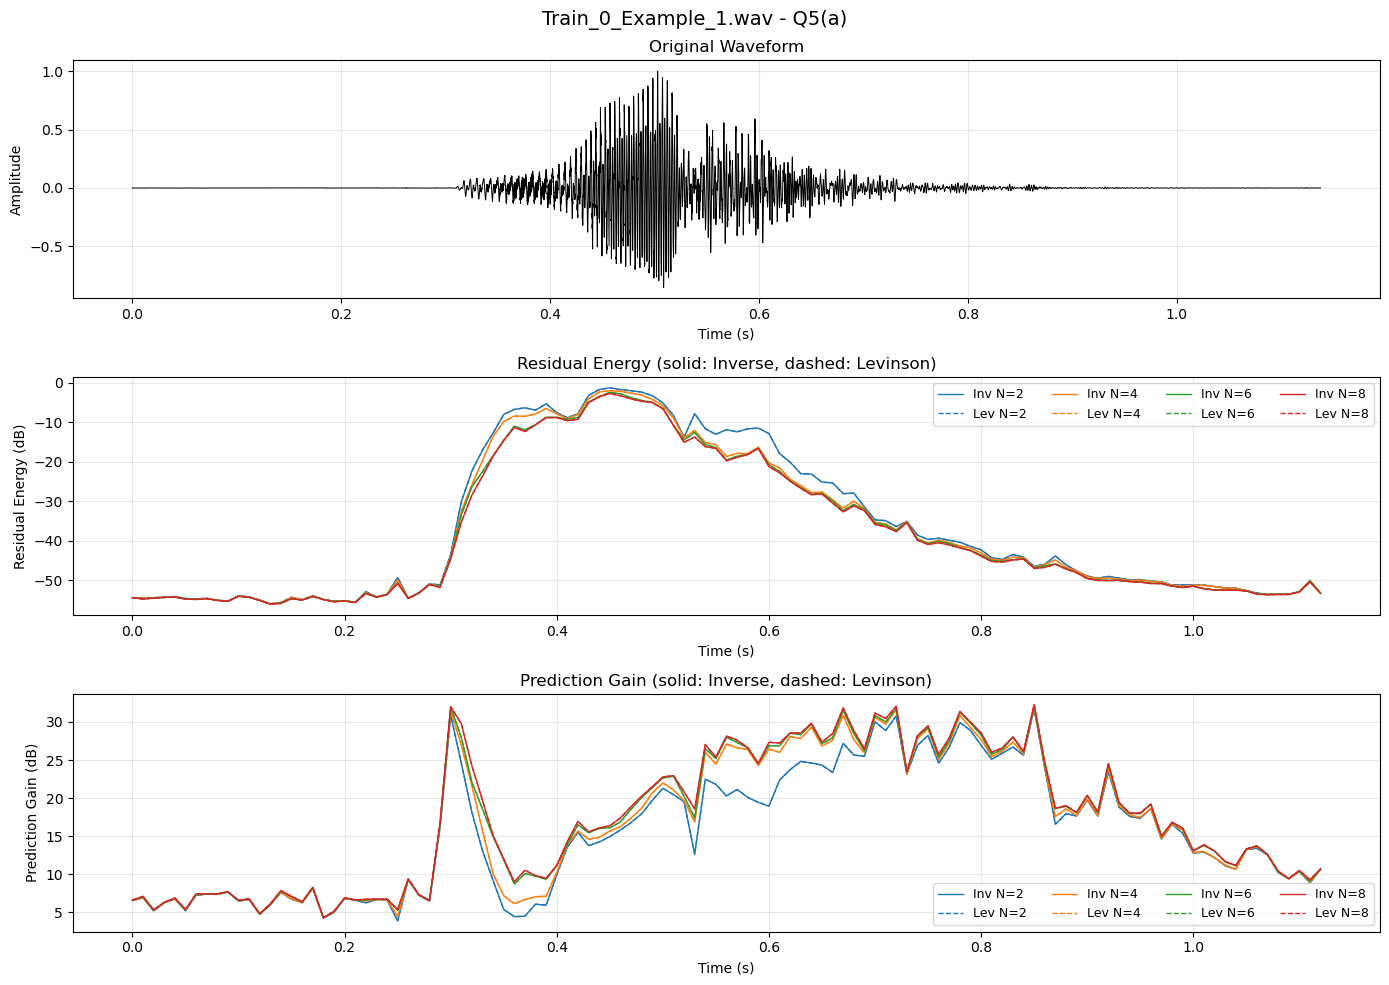
\includegraphics[width=\textwidth]{P5a_ex1.png}
  \caption{Q5(a) -- \texttt{Train\_0\_Example\_1.wav}.
           \textit{Top}: original waveform.
           \textit{Middle}: residual energy (dB) per frame.
           \textit{Bottom}: prediction gain (dB) per frame.
           Solid lines: Inverse method; dashed: Levinson--Durbin.}
  \label{fig:5a_ex1}
\end{figure}

\begin{figure}[H]
  \centering
  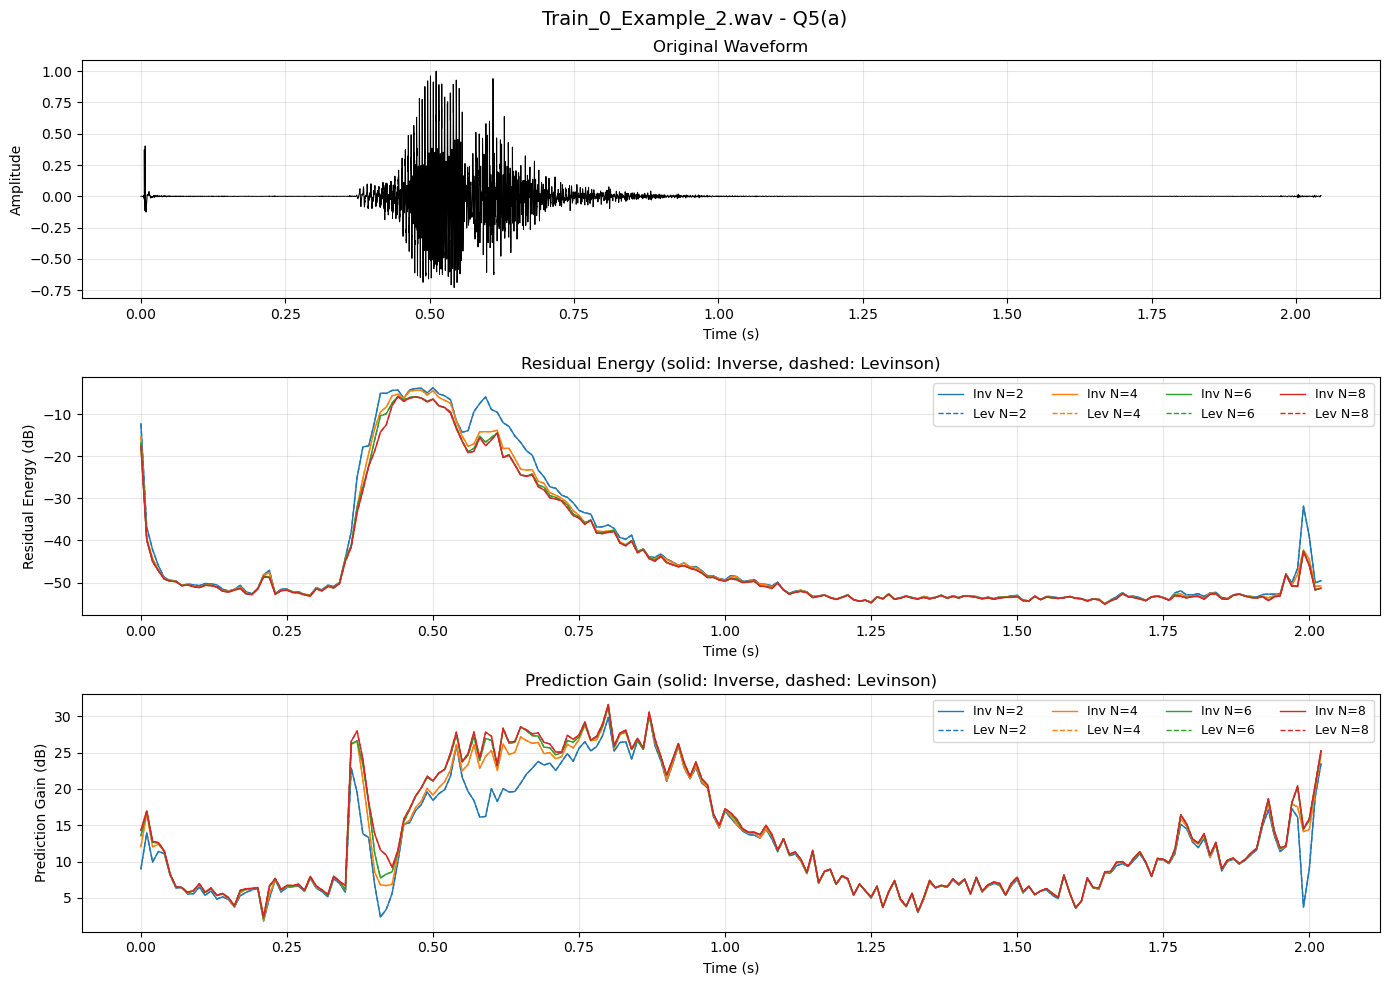
\includegraphics[width=\textwidth]{P05a_ex2.png}
  \caption{Q5(a) -- \texttt{Train\_0\_Example\_2.wav}.}
  \label{fig:5a_ex2}
\end{figure}

\begin{figure}[H]
  \centering
  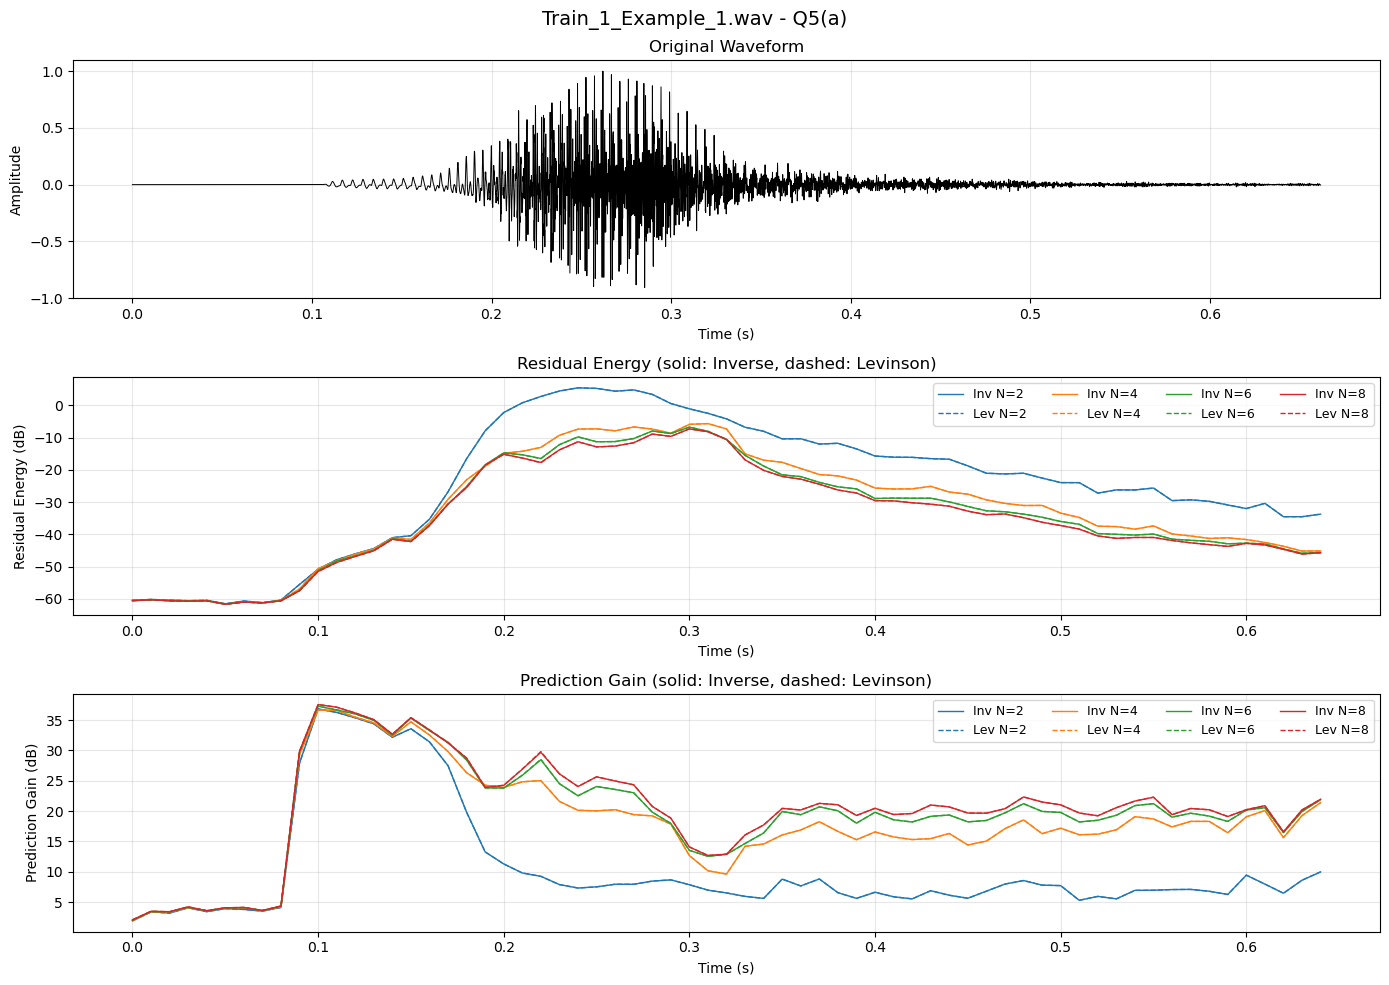
\includegraphics[width=\textwidth]{P05a_ex3.png}
  \caption{Q5(a) -- \texttt{Train\_1\_Example\_1.wav}.}
  \label{fig:5a_ex3}
\end{figure}

\begin{figure}[H]
  \centering
  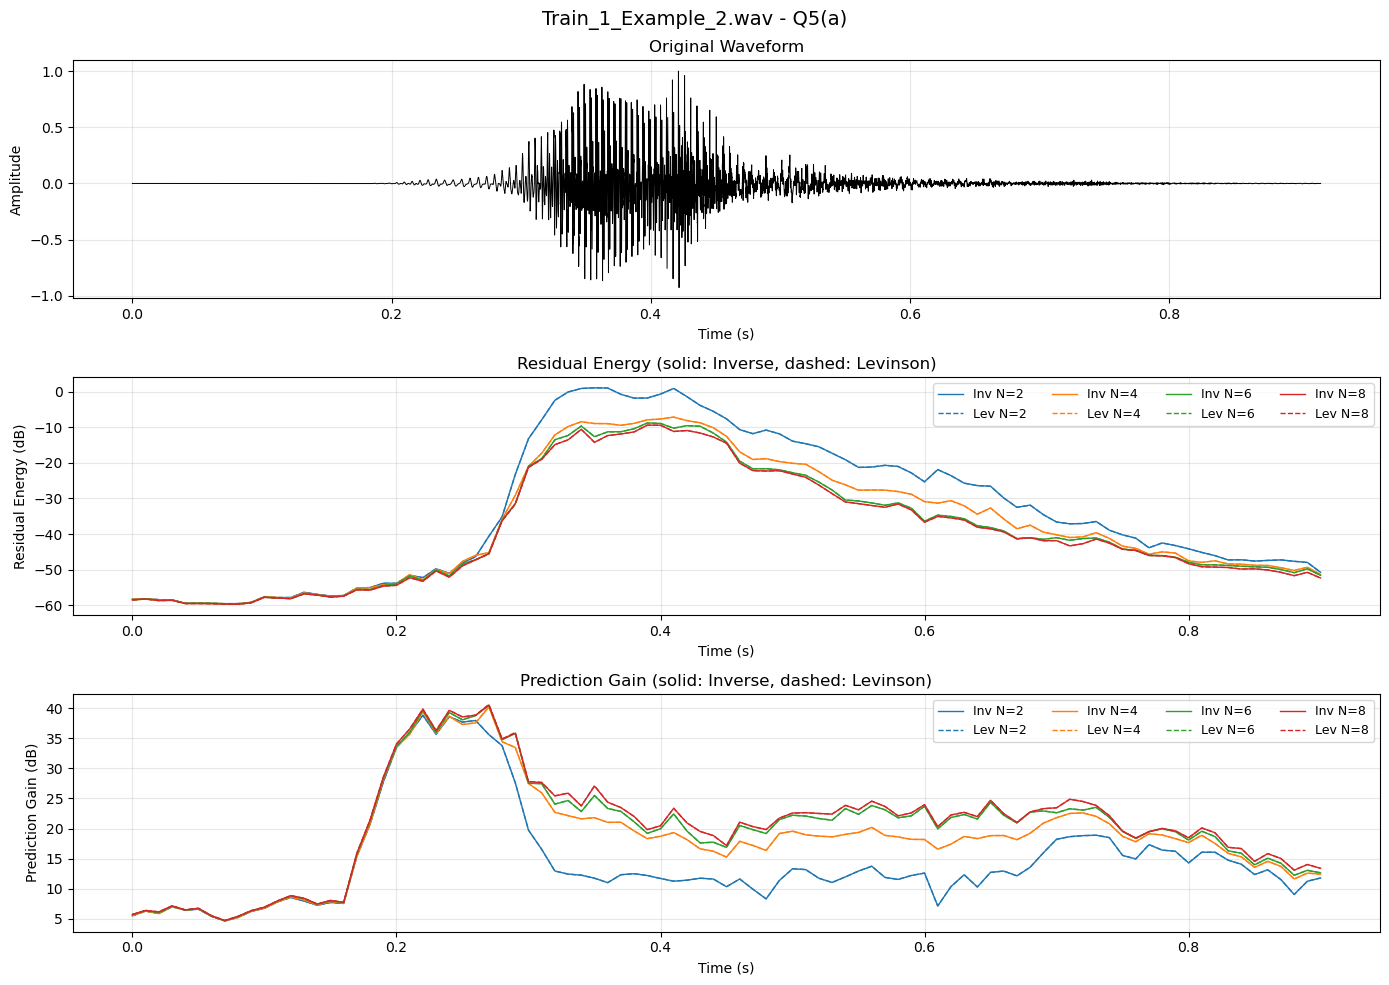
\includegraphics[width=\textwidth]{P05a_ex4.png}
  \caption{Q5(a) -- \texttt{Train\_1\_Example\_2.wav}.}
  \label{fig:5a_ex4}
\end{figure}

\subsubsection*{Observations -- Q5(a)}

\begin{enumerate}
  \item \textbf{Residual energy tracks speech activity.}
        Frames with silence (before or long after the main utterance)
        have very low residual energy ($\lesssim -45$\,dB), whereas
        actively voiced frames have residual energies close to
        $-5$ to $0$\,dB.  This is expected: during silence there is
        almost nothing to predict, so the raw energy is tiny.

  \item \textbf{Voiced vs.\ unvoiced discrimination via prediction gain.}
        Voiced frames exhibit \emph{high prediction gain} (15--40\,dB):
        the quasi-periodic, highly correlated glottal excitation makes the
        spectrum strongly peaked, and LP can model those formant peaks well
        with a small residual. Unvoiced (fricative) frames, whose spectrum
        is nearly flat (noise-like), yield low prediction gain
        ($\approx5$--10\,dB), as LP finds little autocorrelation structure
        to exploit. This connection is key to classic LP-based voiced/unvoiced
        detectors.

  \item \textbf{Higher order $N$ lowers residual energy.}
        Consistent with Eq.~\eqref{eq:monotone}, adding more predictor
        taps always decreases (or at worst preserves) the prediction error
        energy. The improvement from $N=2\to4$ is large; beyond $N=6$
        the gain curves are nearly superimposed, suggesting saturation
        for speech at 16\,kHz (roughly $2$--$3$ formants captured by
        $N=6$--$8$).

  \item \textbf{Inverse method $\approx$ Levinson--Durbin.}
        The solid and dashed curves of each colour are practically
        indistinguishable for all four files: both solvers minimise
        the same quadratic cost (Eq.~\eqref{eq:yw}) and differ only
        in numerical implementation.
\end{enumerate}

% ----------------------------------------------------------
\subsection*{Question 5(b) -- Signal Reconstruction via AR Model}

The AR model reconstructs each frame spectrum as:
\begin{equation}
  \hat{X}(e^{j\omega}) = \sqrt{E_N}\,\frac{1}{A(e^{j\omega})} \cdot e^{j\phi(\omega)},
\end{equation}
where $\phi(\omega)$ is either the \emph{original STFT phase} (true-phase case)
or a \emph{uniformly random phase} (random-phase case).
The inverse STFT reassembles the signal with overlap-add (OLA).

\begin{lstlisting}[caption={Signal reconstruction via overlap-add with original and random phase}]
def reconstruct_signal(frames, starts, frame_len, solver, order, orig_x):
    win   = np.hamming(frame_len)
    n_fft = frame_len;  n_bins = n_fft // 2 + 1
    y_orig, y_rand, win_sum = (np.zeros(starts[-1]+frame_len) for _ in range(3))
    rng = np.random.default_rng(0)

    for i, frame in enumerate(frames):
        s  = starts[i]
        xw = frame * win
        X  = np.fft.rfft(xw, n=n_fft)
        phase      = np.angle(X)
        rand_phase = rng.uniform(-np.pi, np.pi, size=n_bins)

        a, err_var = solver(xw, order)
        den = np.concatenate(([1.0], a))
        _, H = freqz([1.0], den, worN=n_bins)
        mag_env = np.sqrt(max(err_var, EPS)) * np.abs(H)  # AR envelope

        Xo = mag_env * np.exp(1j * phase)          # true phase
        Xr = mag_env * np.exp(1j * rand_phase)     # random phase

        xo = np.fft.irfft(Xo, n=n_fft)[:frame_len]
        xr = np.fft.irfft(Xr, n=n_fft)[:frame_len]

        y_orig[s:s+frame_len] += xo * win
        y_rand[s:s+frame_len] += xr * win
        win_sum[s:s+frame_len] += win**2            # OLA normalisation

    y_orig /= np.maximum(win_sum, EPS)
    y_rand /= np.maximum(win_sum, EPS)
    n = min(len(orig_x), len(y_orig))
    return y_orig[:n], y_rand[:n]
\end{lstlisting}

\subsubsection*{SNR vs.\ LP Order}

\begin{figure}[H]
  \centering
  \begin{subfigure}[b]{0.48\textwidth}
    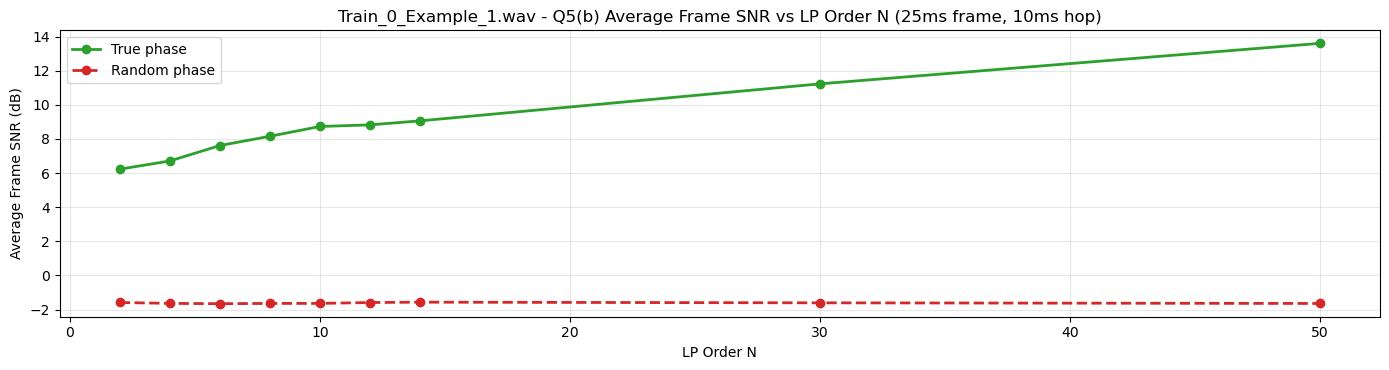
\includegraphics[width=\textwidth]{P05b_snrvslp_ex1.png}
    \caption{\texttt{Train\_0\_Example\_1.wav}}
  \end{subfigure}
  \hfill
  \begin{subfigure}[b]{0.48\textwidth}
    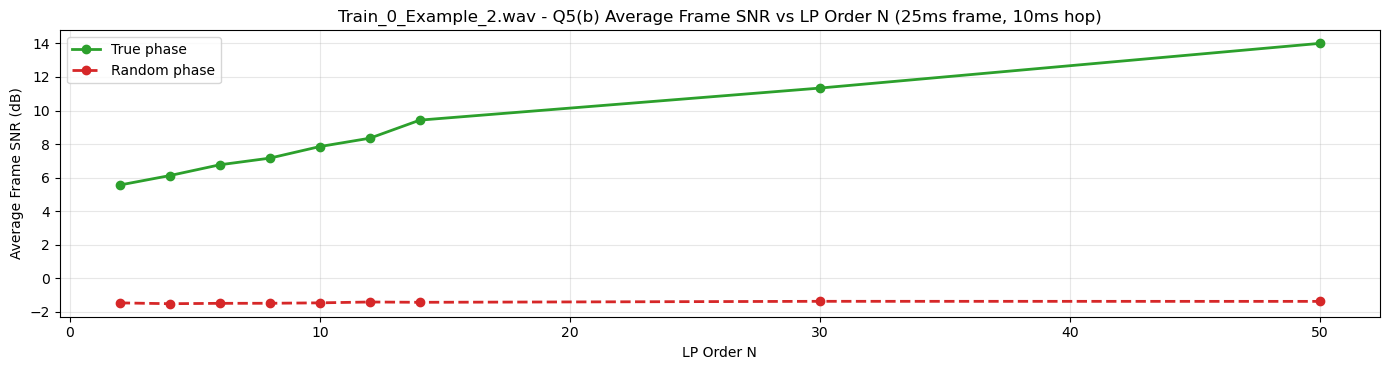
\includegraphics[width=\textwidth]{P05b_snrvslp_ex2.png}
    \caption{\texttt{Train\_0\_Example\_2.wav}}
  \end{subfigure}

  \vspace{0.5em}
  \begin{subfigure}[b]{0.48\textwidth}
    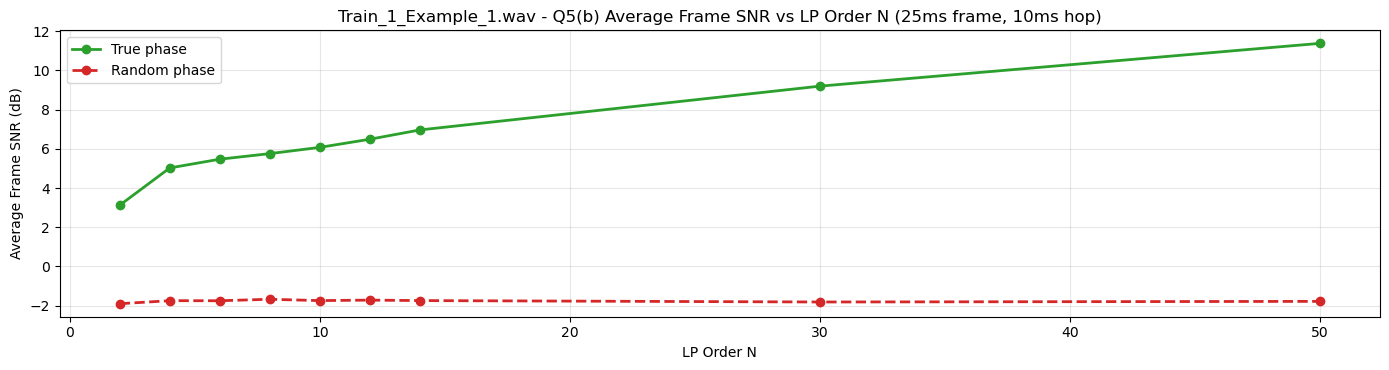
\includegraphics[width=\textwidth]{P05b_snrvslp_ex3.png}
    \caption{\texttt{Train\_1\_Example\_1.wav}}
  \end{subfigure}
  \hfill
  \begin{subfigure}[b]{0.48\textwidth}
    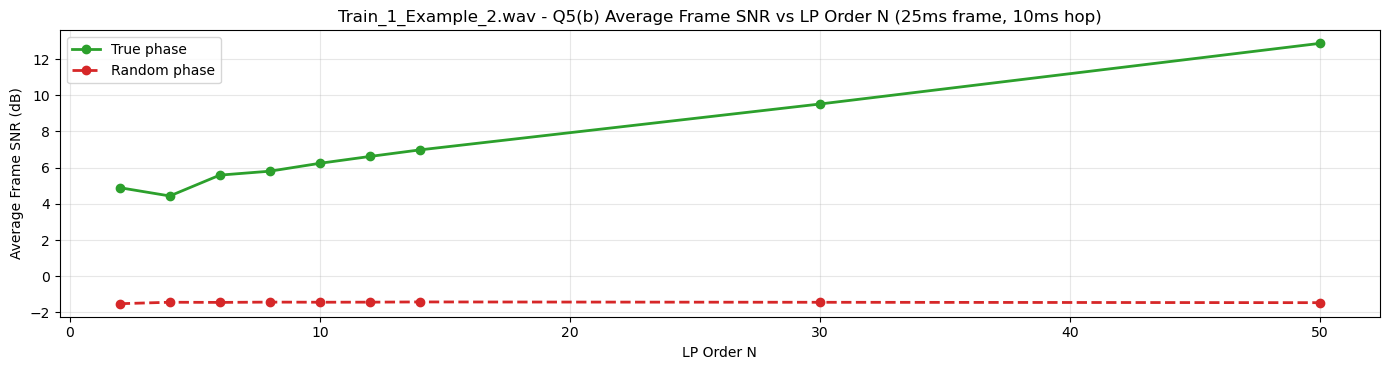
\includegraphics[width=\textwidth]{P05b_snrvslp_ex4.png}
    \caption{\texttt{Train\_1\_Example\_2.wav}}
  \end{subfigure}
  \caption{Q5(b) -- Average frame SNR of AR-reconstructed signal
           vs.\ LP order $N$ for true-phase (green) and random-phase (red)
           excitation.  LP orders tested:
           $N \in \{2,4,6,8,10,12,14,30,50\}$.}
  \label{fig:5b_snr}
\end{figure}

\subsubsection*{Waveform and Spectrogram Comparison ($N=50$)}

\begin{figure}[H]
  \centering
  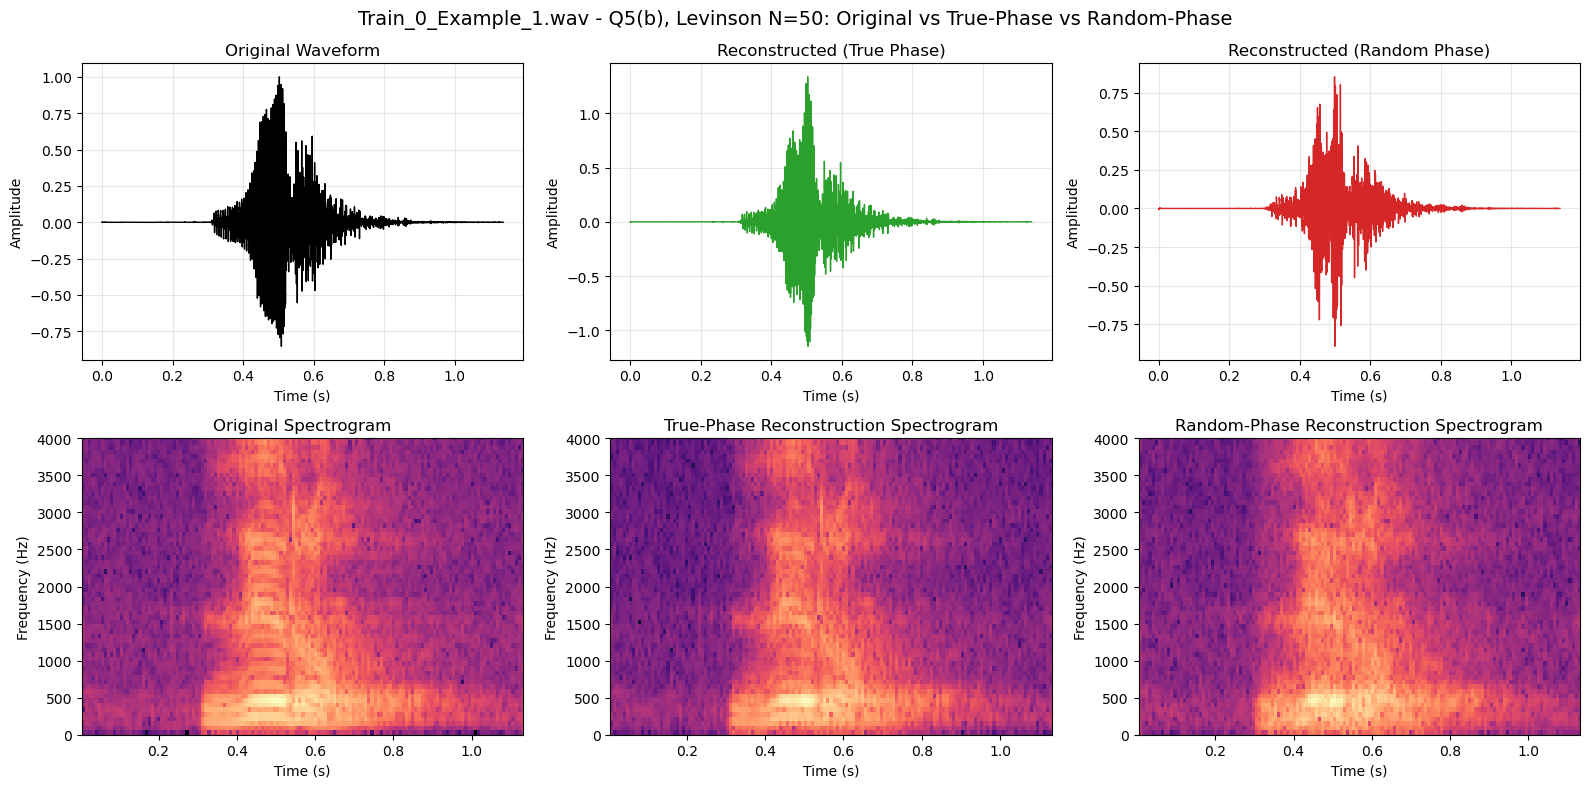
\includegraphics[width=\textwidth]{P05b_stft_ex1.png}
  \caption{Q5(b) -- \texttt{Train\_0\_Example\_1.wav}, Levinson $N=50$.
           \textit{Top row}: original, true-phase, and random-phase
           reconstructed waveforms.
           \textit{Bottom row}: corresponding spectrograms.}
  \label{fig:5b_stft1}
\end{figure}

\begin{figure}[H]
  \centering
  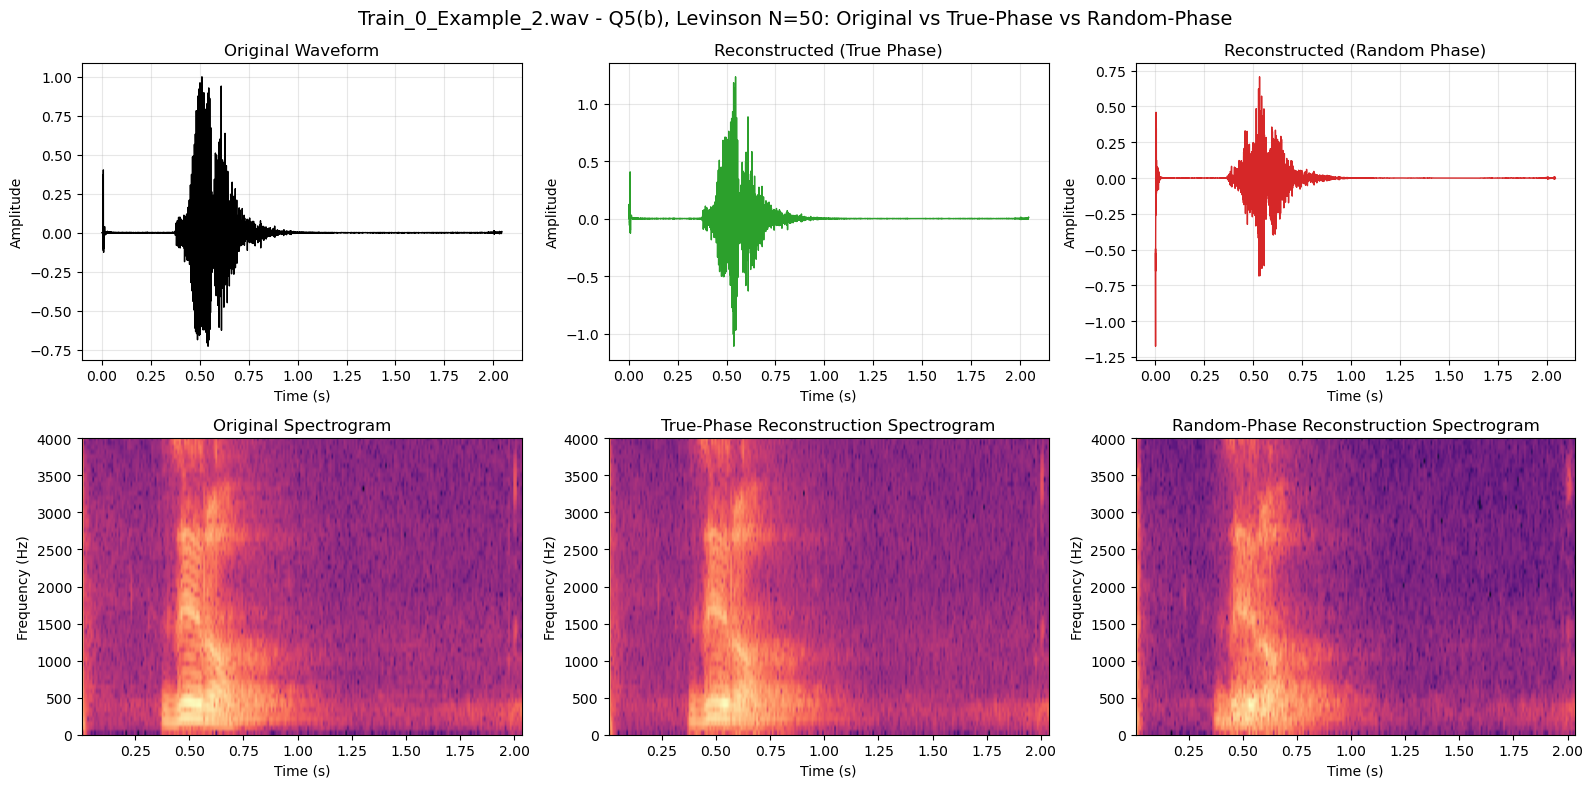
\includegraphics[width=\textwidth]{P05b_stft_ex2.png}
  \caption{Q5(b) -- \texttt{Train\_0\_Example\_2.wav}, Levinson $N=50$.}
  \label{fig:5b_stft2}
\end{figure}

\subsubsection*{Observations -- Q5(b)}

\begin{enumerate}
  \item \textbf{True-phase reconstruction improves with $N$.}
        The average frame SNR for the true-phase case increases
        monotonically from $\approx6$\,dB at $N=2$ to
        $\approx13$\,dB at $N=50$ across all four files
        (Fig.~\ref{fig:5b_snr}).
        The slope is largest for small $N$ (where adding one more pole
        adds a new formant) and flattens beyond $N\approx15$, suggesting
        that eight or so poles capture most of the spectral envelope
        information. No strict saturation is observed up to $N=50$.

  \item \textbf{Random-phase reconstruction is consistently $\approx-1.5$\,dB SNR.}
        Scrambling the spectral phase destroys temporal fine structure
        (the glottal pulses), resulting in a noisy, breathy output whose
        SNR barely changes with $N$.  This shows that for a \emph{waveform}
        fidelity metric the phase is at least as important as the spectral
        envelope.

  \item \textbf{Spectrograms reveal what SNR does not.}
        Even though the random-phase reconstructed signal has very low SNR,
        its spectrogram (Figs.~\ref{fig:5b_stft1}--\ref{fig:5b_stft2})
        preserves the formant structure (horizontal bands) quite well.
        This reflects the fact that LP correctly models the spectral
        \emph{envelope}; it is only the excitation (voiced periodicity)
        that is lost.

  \item \textbf{True-phase reconstruction preserves pitch structure.}
        The true-phase waveform shows clear glottal pulse patterns in
        voiced regions (visible as periodic spikes), while the random-phase
        version produces a smoothed, diffuse envelope -- similar to
        whispering or spectrally shaped noise. This dichotomy is the
        basis for LP vocoders.

  \item \textbf{Quality does not \emph{saturate} quickly.}
        Unlike the residual energy (Q5a) which plateaus by $N\approx8$,
        reconstruction SNR continues to grow noticeably between
        $N=14$ and $N=50$. This is because SNR measures absolute
        waveform differences, which are reduced by finer spectral
        envelope fitting even when the perceptual improvement is small.
\end{enumerate}

% ==========================================================
\questionheader{6. Spectral Transform Linear Prediction (STLP)}

\subsection*{Formulation}

Standard LP ($q=1$) solves the Yule--Walker system using the autocorrelation
sequence of $x[n]$, which equals the inverse DTFT of $S_{xx}(e^{j\omega})$.
The \textbf{Spectral Transform LP} generalises this by computing the
modified autocorrelation as the inverse DTFT of $S_{xx}^{1/q}(e^{j\omega})$:
\begin{equation}
  \tilde{r}_q[k] = \text{IDTFT}\!\left\{S_{xx}(e^{j\omega})^{1/q}\right\}
                  = \frac{1}{2\pi}\int_{-\pi}^{\pi}
                    S_{xx}(e^{j\omega})^{1/q}\,e^{j\omega k}\,d\omega.
  \label{eq:stlp_acf}
\end{equation}
Solving the Yule--Walker system with $\tilde{r}_q[k]$ yields LP coefficients
$\hat{a}^{(q)}$ and residual variance $\hat{E}_q$, giving the AR model of
$S_{xx}^{1/q}$:
\begin{equation}
  \hat{S}^{1/q}_{xx}(e^{j\omega}) = \frac{\hat{E}_q}{\left|A_q(e^{j\omega})\right|^2}.
  \label{eq:stlp_model}
\end{equation}
Raising to the power $q$ recovers the estimate of the original PSD:
\begin{equation}
  \hat{S}_{xx}(e^{j\omega}) = \left[\hat{S}^{1/q}_{xx}(e^{j\omega})\right]^q
                            = \left[\frac{\hat{E}_q}{\left|A_q(e^{j\omega})\right|^2}\right]^q.
  \label{eq:stlp_psd}
\end{equation}
For $q=1$ this reduces to the standard LP PSD of Eq.~\eqref{eq:arpsd}.
Increasing $q$ effectively \emph{compresses} the spectral dynamic range
before fitting, encouraging the LP model to allocate poles uniformly
across frequency rather than only at the strongest formants.

\begin{lstlisting}[caption={STLP implementation (\texttt{transform\_lp})}]
def transform_lp(frame, fs, order, q):
    xw  = frame * win
    xw /= np.sqrt(np.sum(win**2) + EPS)          # normalise by window energy

    X   = np.fft.fft(xw)
    Sxx = np.abs(X)**2
    Sxx = Sxx / (np.max(Sxx) + EPS)              # numerical stability

    S_q  = Sxx ** (1.0 / q)                      # power-law compression
    r_q  = np.real(np.fft.ifft(S_q))             # modified autocorrelation

    a, err = yw_from_acf(r_q, order)             # Yule-Walker solve

    A       = np.fft.fft(np.concatenate(([1.], a)), n=len(Sxx))
    S_q_hat = err / (np.abs(A)**2 + EPS)         # AR model of S^{1/q}

    S_hat   = np.maximum(S_q_hat, EPS) ** q      # raise to power q

    f    = np.fft.rfftfreq(len(Sxx), 1/fs)
    half = len(f)
    return f, Sxx[:half], S_hat[:half]
\end{lstlisting}

\subsection*{Frame Selection}

A voiced and an unvoiced frame are selected from
\texttt{Train\_0\_Example\_1.wav} using the Levinson residual energy
profile (order $N=8$) as a proxy: the frame with \emph{minimum}
residual energy is deemed voiced (strong glottal correlation allows
accurate prediction), and the frame with \emph{maximum} residual energy
is unvoiced (noise-like spectrum, poor predictability).

\begin{figure}[H]
  \centering
  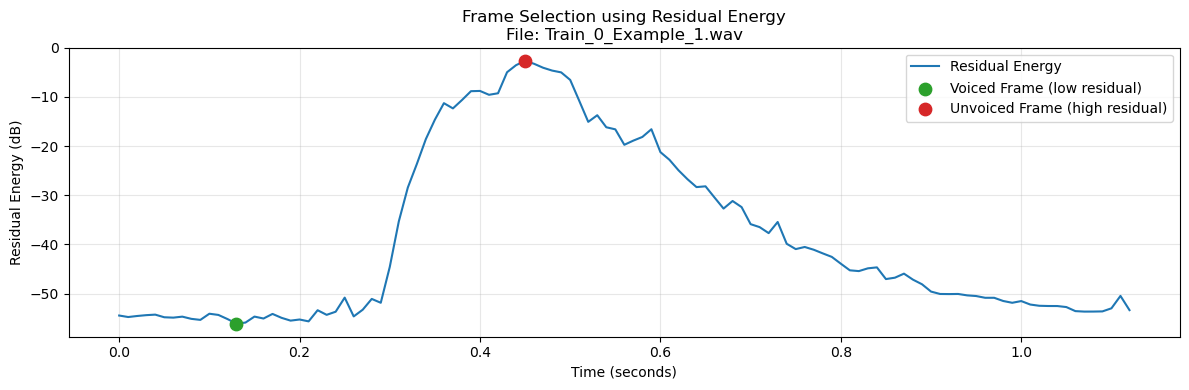
\includegraphics[width=\textwidth]{P06_location_voiced_unvoiced.png}
  \caption{Frame selection using residual energy profile.
           The green dot marks the selected voiced frame (near silence
           onset, very low residual); the red dot marks the selected
           unvoiced frame (peak of speech activity -- highest residual).}
  \label{fig:q6_frames}
\end{figure}

\noindent\textit{Note on frame labelling:} The green dot (minimum residual energy)
falls in the pre-speech silence region.  During silence the signal is near zero,
so the LP residual is also nearly zero -- this is why the algorithm picks it.
In practice, voiced/unvoiced detection should be applied only within speech
activity regions; here it serves to illustrate the two extremes of residual energy.

\subsection*{PSD Estimation for $q = 1, 2, 3$}

\begin{figure}[H]
  \centering
  
\includegraphics[width=\textwidth]{P06.png}
  \caption{Q6 -- Transform LP PSD estimates for $q = 1, 2, 3$
           and AR order $N=10$.
           \textit{Top row}: voiced frame.
           \textit{Bottom row}: unvoiced frame.
           Black: true PSD; green/red dashed: $\hat{S}_{xx}$ from STLP.}
  \label{fig:q6_psd}
\end{figure}

\subsubsection*{Observations -- Q6}

\begin{enumerate}
  \item \textbf{$q=1$ (standard LP) focuses on high-energy regions.}
        Because the Yule--Walker system is solved directly on the raw PSD,
        the AR model allocates its poles to match the dominant spectral
        peaks (formants in voiced frames, or broadband energy in unvoiced frames).
        For voiced frames the estimate captures the two or three largest
        formant peaks but can miss lower-energy formants or valley regions.

  \item \textbf{$q=2$ compresses the PSD dynamic range.}
        Taking the square root of the PSD ($S_{xx}^{1/2}$) before solving
        attenuates the dominance of the strongest spectral peaks.
        As a result, the AR model distributes its poles more evenly across
        the spectrum. The estimate for voiced frames shows a somewhat
        smoother envelope that better follows medium-energy formants,
        though the peak heights are less accurately captured.

  \item \textbf{$q=3$ leads to over-smoothing.}
        The cube-root compression ($S_{xx}^{1/3}$) strongly suppresses
        high-energy peaks. The resulting LP model fits the compressed
        spectrum well, but after the $(\cdot)^3$ inverse transform the
        estimated PSD tends to be nearly flat (over-smoothed).
        For voiced frames, formant peaks are essentially washed out;
        for unvoiced frames (which are already flatter), the estimate
        is comparable to $q=1$.

  \item \textbf{Voiced vs.\ unvoiced frames respond differently.}
        For the \emph{voiced} frame, $q=1$ gives the sharpest and most
        interpretable formant peaks. As $q$ increases the model loses
        the ability to resolve fine spectral detail because the
        compression brings all frequency bins to similar amplitudes.
        For the \emph{unvoiced} frame the spectrum is already
        relatively flat, so varying $q$ has a smaller effect --
        all three models produce roughly similar, smooth PSD estimates.
\end{enumerate}



\end{document}
